\section{8.37}

\paragraph{Specification}
A Lamp with the weight $F_G = |\vec{F_G}| = 45 N$ should be mounted to a vertical wall with 
the help of to rods $s_1$ and $s_2$.

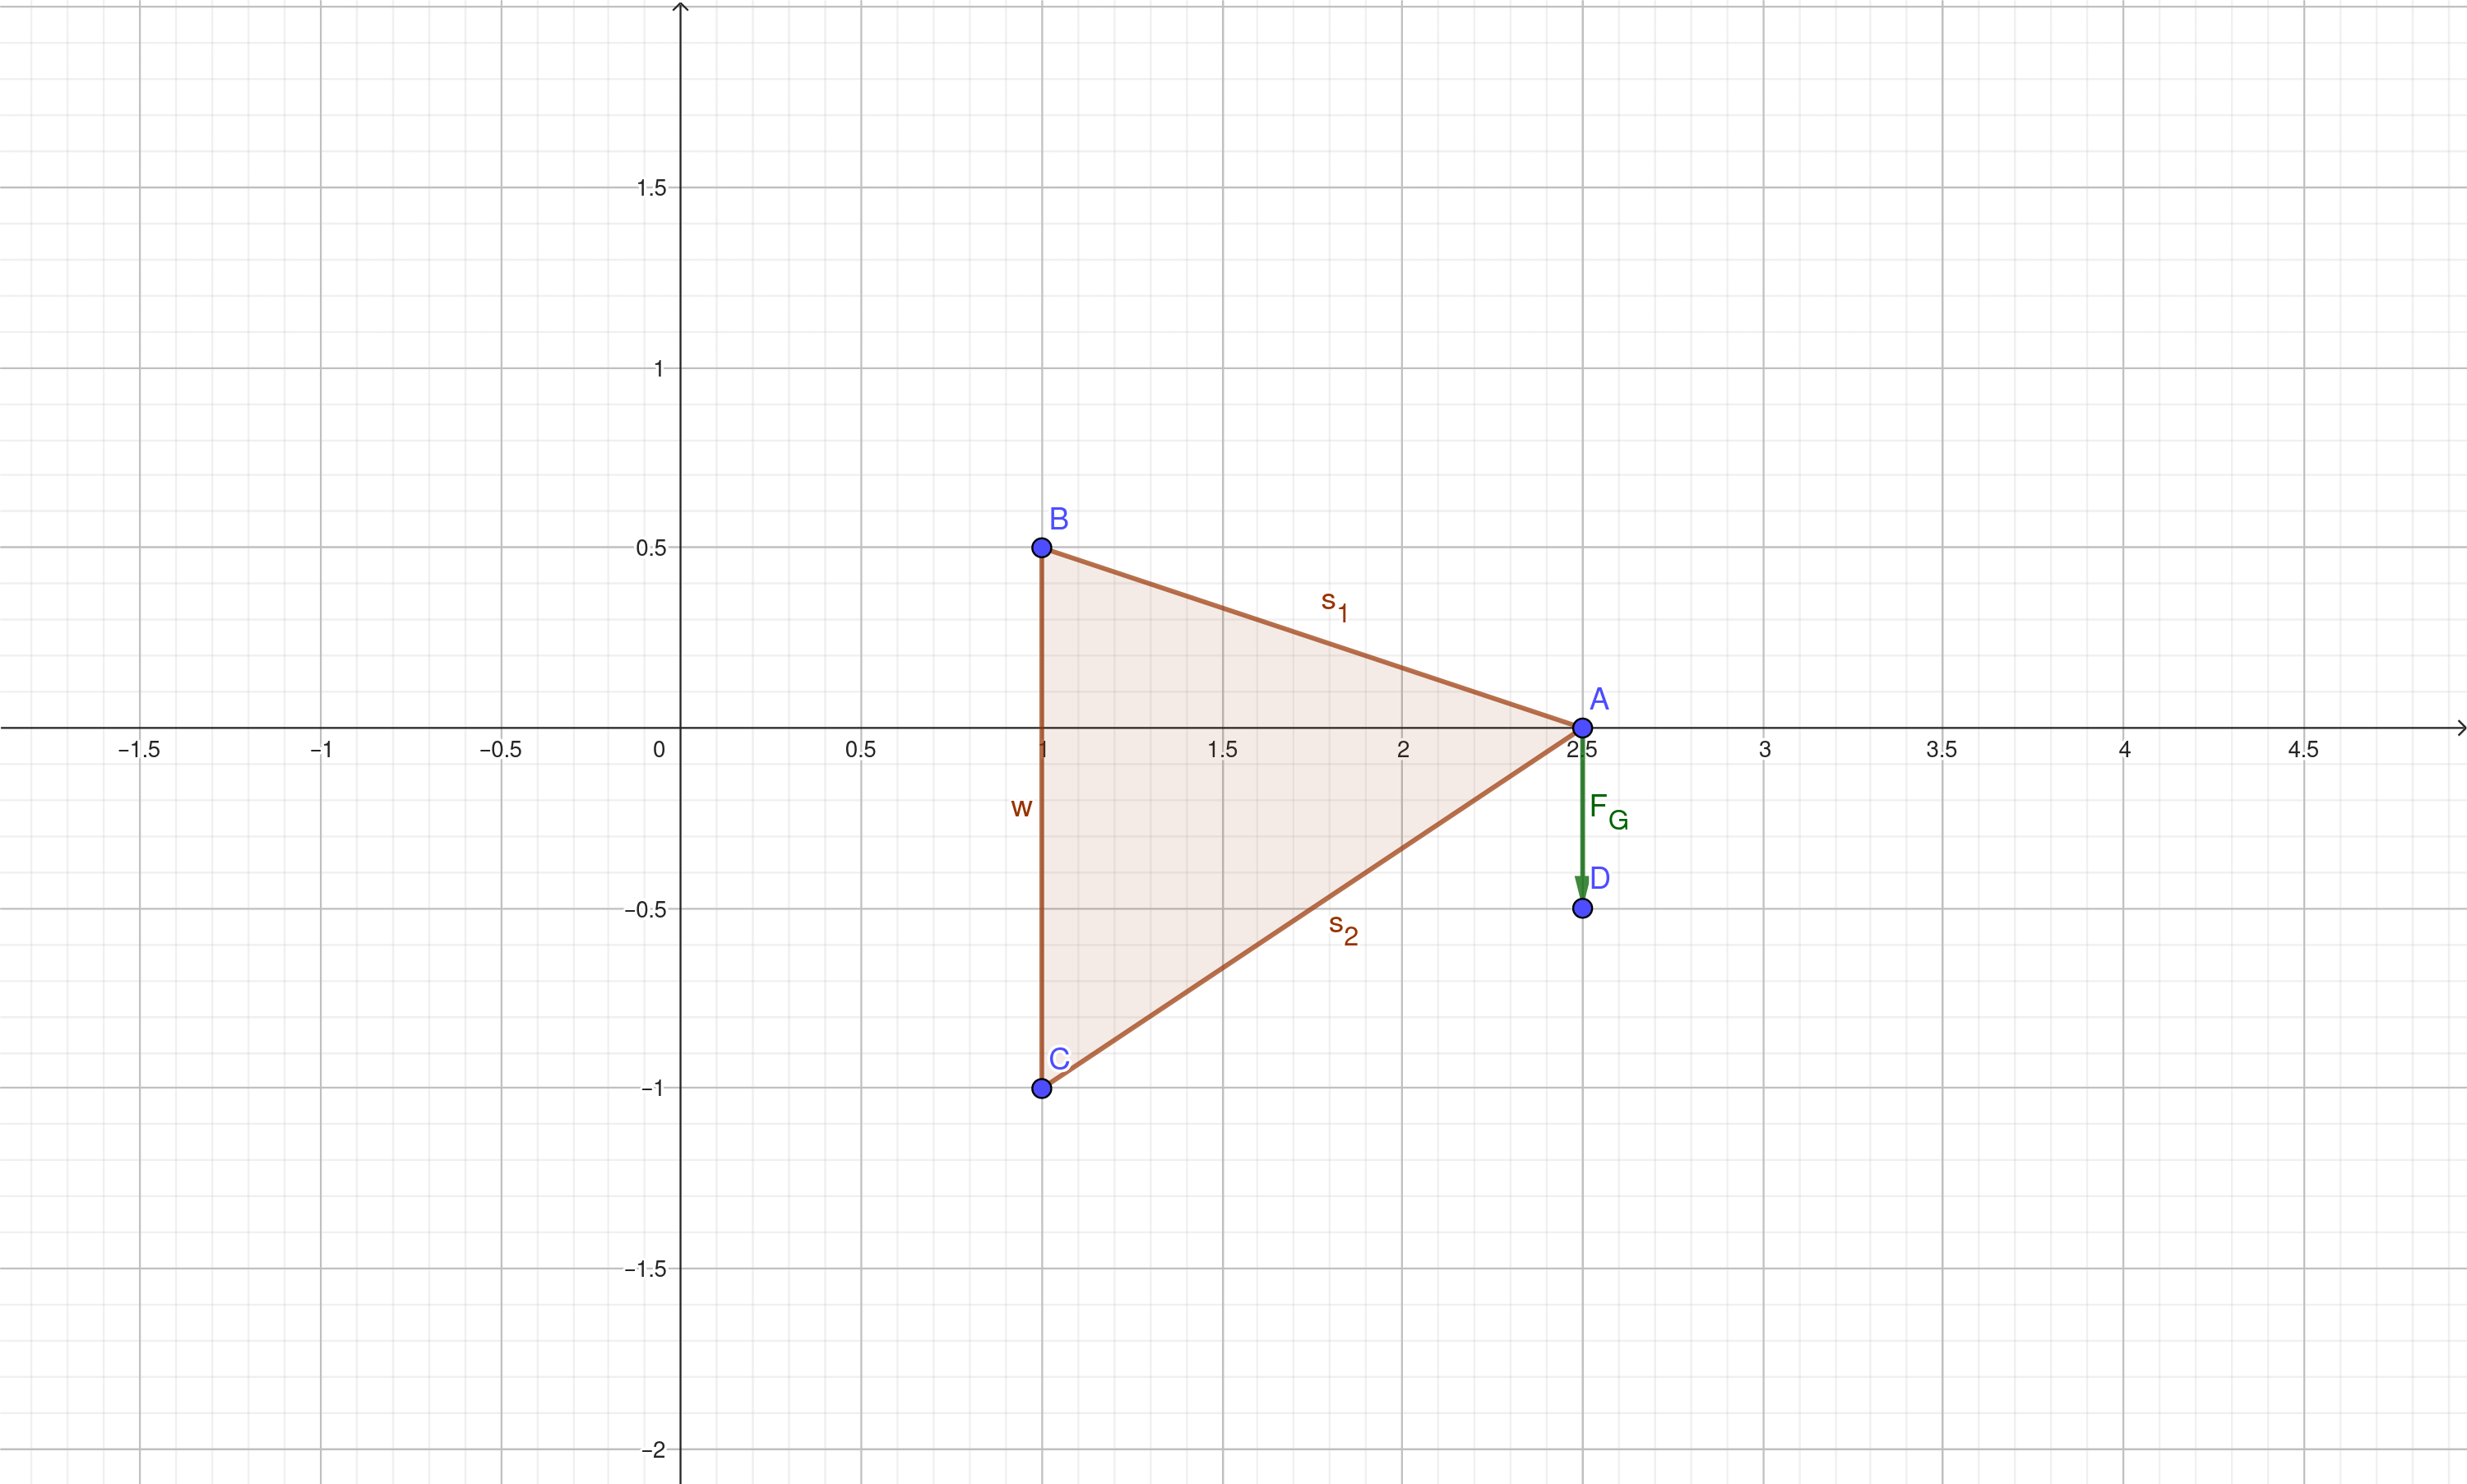
\includegraphics[width=\linewidth]{images/8-37-1.png}

\subsection{1)}
\paragraph{Requirements:}
Sketch the force triangle of the forces acting on the point $A$ where the lamp is mounted.
Denote the directions of the forces.

\paragraph{Answer:}
The direction of the force $\vec{F_1}$ is taken from the direction of $s_1 = \begin{pmatrix}
   -1.5 \\ 
   0.5
\end{pmatrix}$. \\
The same goes for the force $\vec{F_2}$: $s_2 = \begin{pmatrix}
   1.5 \\ 
   1
\end{pmatrix}$. \\
The weight force points vertically down with $45 N$: $\vec{F_G} = \begin{pmatrix}
   0 \\ 
   -45
\end{pmatrix}$.

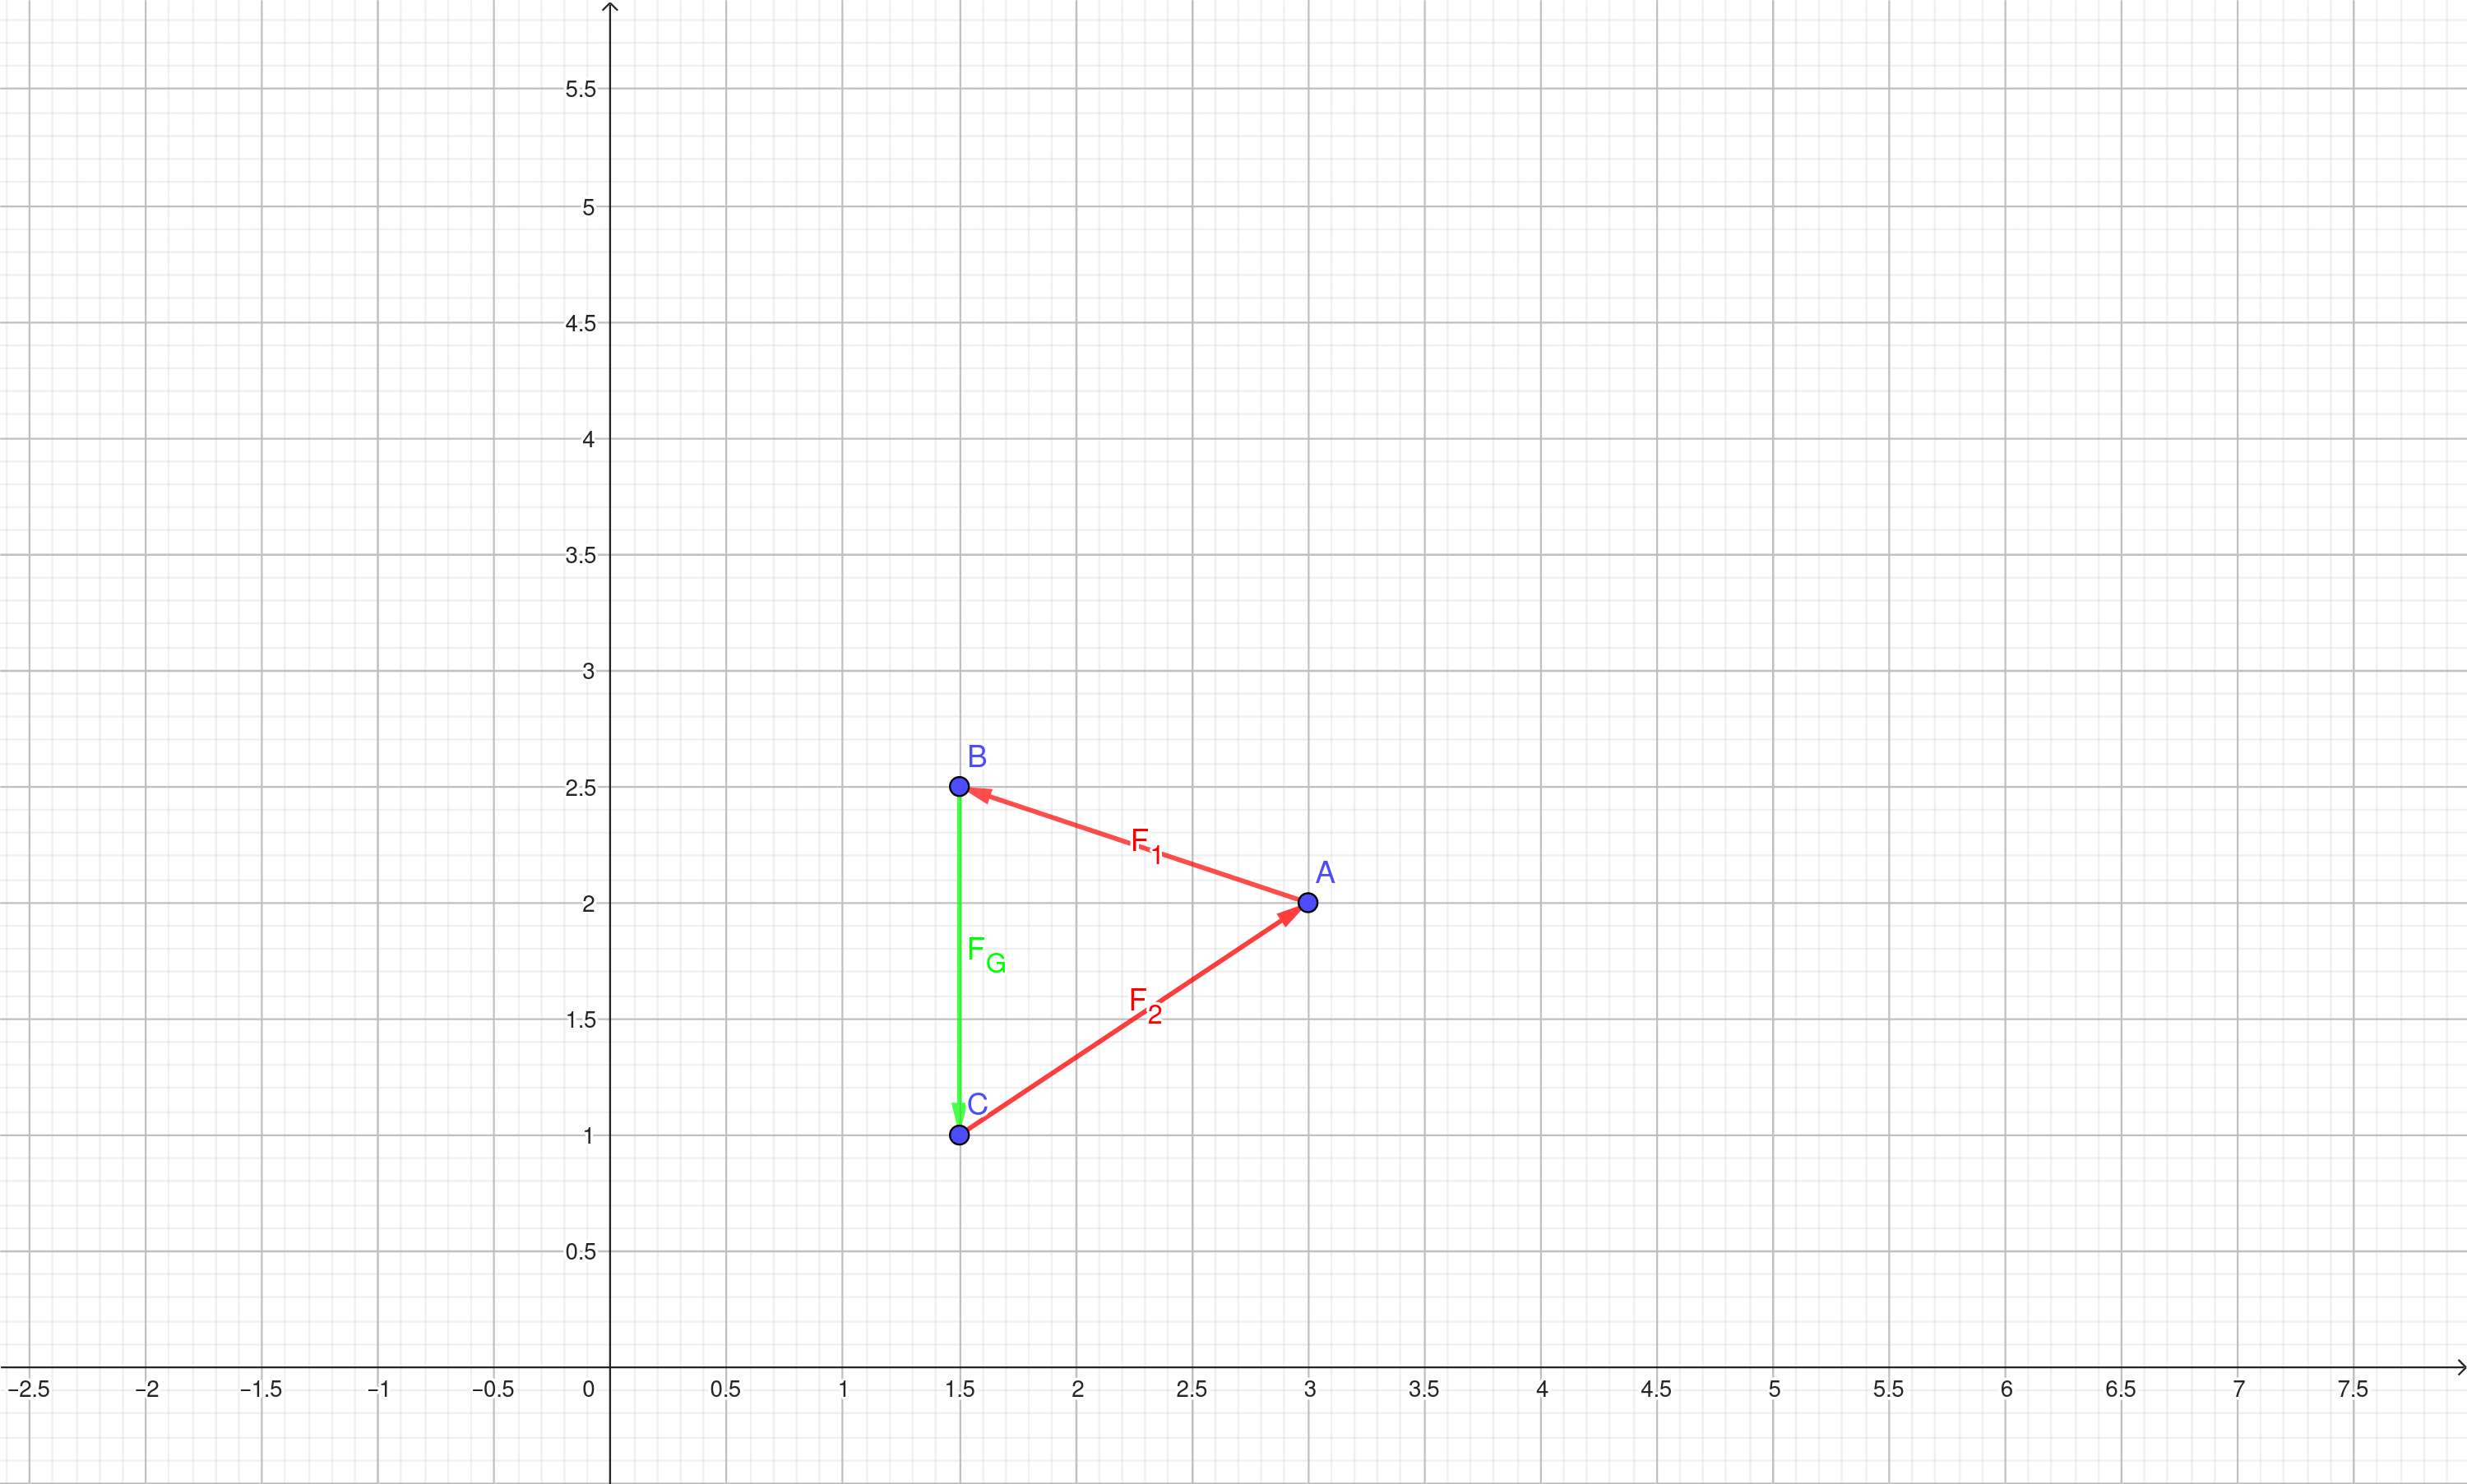
\includegraphics[width=\linewidth]{images/8-37-2.png}

\subsection{2)}
\paragraph{Requirements:}
Calculate the magnitudes of the forces in the rods  $s_1$ and $s_2$. \\ 
Note: The sum of the forces acting on $A$ has to be the zero vector.

\begin{align}
   \vec{F_G} + \vec{F_1} + \vec{F_2} &= \begin{pmatrix}
       0 \\ 
       0
   \end{pmatrix} \\
   \vec{F_1} + \vec{F_2} &= -\vec{F_G} \\
   r * \begin{pmatrix}
       -1.5 \\ 
       -.5
   \end{pmatrix} + t * \begin{pmatrix}
       1.5 \\ 
       1 
   \end{pmatrix} &= \begin{pmatrix}
       0 \\  
       45
   \end{pmatrix}
\end{align} \\
I.  $-1.5r + 1.5t = 0 \Rightarrow t = r$ \\
II. $0.5r + t = 45$ \\
I. in II.   $1.5r = 45 \Rightarrow r = 30, t = 30$

\begin{align}
   \vec{F_1} &= r + s_1 = \begin{pmatrix}
       -45  \\
       15
   \end{pmatrix} \\
   |\vec{F_1}| &= 47.343... N \approx 47N \\[20pt]
   \vec{F_2} &= r + s_2 = \begin{pmatrix}
       45  \\
       30
   \end{pmatrix} \\
   |\vec{F_2}| &= 54.083... N \approx 54N
\end{align}
